% This is samplepaper.tex, a sample chapter demonstrating the
% LLNCS macro package for Springer Computer Science proceedings;
% Version 2.21 of 2022/01/12
%
\documentclass[runningheads]{llncs}
%
\usepackage[T1]{fontenc}
% T1 fonts will be used to generate the final print and online PDFs,
% so please use T1 fonts in your manuscript whenever possible.
% Other font encondings may result in incorrect characters.
%
\usepackage{graphicx}
% Used for displaying a sample figure. If possible, figure files should
% be included in EPS format.
%
% If you use the hyperref package, please uncomment the following two lines
% to display URLs in blue roman font according to Springer's eBook style:
%\usepackage{color}
%\renewcommand\UrlFont{\color{blue}\rmfamily}
%\urlstyle{rm}
\usepackage{comment}
\usepackage{diagbox}
\usepackage{url}
%\usepackage{breakurl}
\usepackage[breaklinks]{hyperref}

\usepackage[T1]{fontenc}
\usepackage{soul}
\usepackage{graphicx}
\usepackage{amsmath}
\usepackage{booktabs}
\usepackage{pifont}
\usepackage{enumitem}
\usepackage{tikz}
\usepackage{cite}
\usepackage{amsmath,amssymb,amsfonts}
\usepackage{algorithmic}
\usepackage{graphicx}
\usepackage{textcomp}
\usepackage{xcolor}
\usepackage{amsmath}
\def\BibTeX{{\rm B\kern-.05em{\sc i\kern-.025em b}\kern-.08em
    T\kern-.1667em\lower.7ex\hbox{E}\kern-.125emX}}
    
\def\checkmark{\tikz\fill[scale=0.4](0,.35) -- (.25,0) -- (1,.7) -- (.25,.15) -- cycle;} 

\usetikzlibrary{trees,arrows}

\newlist{todolist}{itemize}{2}
\setlist[todolist]{label=$\square$}
\newcommand{\cmark}{\ding{51}}%
\newcommand{\xmark}{\ding{55}}%
\newcommand{\done}{\rlap{$\square$}{\raisebox{2pt}{\large\hspace{1pt}\cmark}}%
\hspace{-2.5pt}}
\newcommand{\wontfix}{\rlap{$\square$}{\large\hspace{1pt}\xmark}}

\def\UrlBreaks{\do\/\do-}

\renewcommand\thesection{\arabic{section}} % arabic numerals for the sections


% correct bad hyphenation here
\hyphenation{op-tical net-works semi-conduc-tor IEEEconf}
\begin{document}
%% Example cover page for a two-page IEEE conference document
%\onecloumn
% Cover page

\begin{center}
  \textbf{recovery testbed}
\end{center}

\begin{itemize}
  \item DEADLINE: Abstract April 11, Paper April 18, 2025
  \item Publication Venue: QEST+FORMATS 2025
  \item Url for Publication Venue: \url{https://www.qest-formats.org/}
  \item Submission Category or Track:
    \begin{itemize}
        \item Models and metrics for the correctness, performance, reliability, safety, and security of systems (stochastic, probabilistic, and non-deterministic models including Markov chains, automata, Petri nets, process algebra, max-plus algebra, and their variations);
    \end{itemize}
  \item Page limit:  16 pages; currently at 16
  \item Research Contribution: 
   The proposed model enables comparisons of alternative
repair schemes by considering the availability of repair crews,
predicting failure propagation, and estimating the level of
service capacity over time. The model can also guide staffing
decisions by identifying the minimum number of repair crews
required to maintain a particular service level.
\end{itemize}

\vspace{2ex}

%SSS- This helps us keep track of the number of drafts
\textbf{Version 1.1}
Last Updated: 4/1/2025 \\
\textbf{Major Changes Since Previous Draft}
\begin{itemize}
    \item Case study
    \item Conclusion
\end{itemize}

\vspace{2ex}

\textbf{Outline}
\begin{enumerate}
%SSS - Include the number of pages in your current draft in front of each section (not subsection) title. Also include the status (complete, pending, not written).
  %SSS - The following sections should be in every paper. 
  \item  Abstract
  \item Introduction 
  \begin{enumerate}
          \item Blackout in Kenya
          \item Motivation for this paper
          \item Intro to this model
        \end{enumerate}
  \item Related work
  \begin{enumerate}
          \item Modeling of cascading failure
          \item Modeling of the Recovery process
        \end{enumerate}
  \item Proposed recovery model
  \begin{enumerate}
          \item Modeling of Cascading failure
          \begin{enumerate}
              \item States
              \item Actions
              \item Rewards
              \item Transition probabilities
          \end{enumerate}
          \item Repair schemes
          \begin{enumerate}
              \item Randomized priorities
              \item pre-made repair priorities
              \item Look-ahead dynamic priorities
              \item cascading effect dynamic priorities
          \end{enumerate}
        \end{enumerate}
  \item case studies
  \begin{enumerate}
          \item IEEE-14
          \item Simulation Environment
          \item IEEE-14 Failure Cases
          \begin{enumerate}
            \item experiment 1
            \item experiment 2
            \item Experiment 3
            \end{enumerate}
        \item Discussion of results
        \end{enumerate}
  \item Conclusion and Future Work 
    \begin{enumerate}
          \item The contribution to the body of knowledge 
          \item social impact 
          \item future directions, enable advances in the repair scheme area
        \end{enumerate}
  \item Acknowledgements 
  %SSS - Include this text in your acknowledgments: The authors gratefully acknowledge funding from NSF DUE-1742523, DEd GAANN awards P200A180095 and P200A210121, and the Missouri S\&T Intelligent Systems Center.
  \item References
\end{enumerate}

\vspace{2ex}

\textbf{TO DO (Advisors):}
\begin{itemize}
    \item review the paper
\end{itemize}

\textbf{TO DO (Sanfan):}
\begin{itemize}
    \item review the paper entirely
    \item submit for publication 
\end{itemize}

\textbf{Author guidelines (submission requirements)}: \\ 
\url{https://www.qest-formats.org/cfp.html}\\
Regular papers must not exceed 16 pages, excluding references.
We are considering additional presentation-only submission types; details will be provided in the later CfPs.

All papers must be submitted in Springer’s LNCS format and will undergo a rigorous single-blind review process. All submitted papers must be unpublished and not be submitted for publication elsewhere. Papers should be submitted electronically using EasyChair at this link.

Springer encourages authors to include their ORCIDs in their papers. Authors should consult Springer’s authors’ guidelines and use Springer’s LaTeX templates for the preparation of their papers. Submitted papers not complying with the above guidelines may be rejected without undergoing review.
We are considering awards for best papers and best artifacts.

Publications\\
All accepted papers need to be presented and discussed at the conference by one of the authors. The QEST+FORMATS 2025 proceedings will be published in the Springer LNCS series indexed by ISI Web of Science, Scopus, ACM Digital Library, dblp, Google Scholar. All submitted papers will be evaluated by at least three reviewers on the basis of their originality, technical quality, scientific or practical contribution to the state of the art, methodology, clarity, and adequacy of references.

Special Issue\\
We are working on a special issue in a Q1 journal. A selection of the best papers will be invited to submit an extended version of their work to special issues in internationally recognized journals.

Artifact Evaluation\\
Reproducibility of experimental results is crucial to foster an atmosphere of trustworthy, open, and reusable research. To improve and reward reproducibility, QEST+FORMATS 2025 will include a dedicated Artifact Evaluation (AE). Submission of an artifact is mandatory for tool papers (both regular and short), and optional but encouraged for research and case study papers where it can support the results presented in the paper. More details can be found in the corresponding page
%End Cover Sheet


%
\title{A Markov decision process for dynamic scheduling of recovery tasks during cascading failure}
%
%\titlerunning{Abbreviated paper title}
% If the paper title is too long for the running head, you can set
% an abbreviated paper title here
%
\author{Sanfan Liu\orcidID{0000-0002-5089-3500} \and
Sahra Sedigh Sarvestani\orcidID{0000-0002-2917-5643 } \and
Ali R. Hurson\orcidID{0000-0002-9510-0762}}
%
\authorrunning{S. Liu et al.}
% First names are abbreviated in the running head.
% If there are more than two authors, 'et al.' is used.
%
\titlerunning{MDP for scheduling recovery task during cascading failure} %change page header title (short title)

\institute{Missouri University of Science and Technology \\
\email{\{slbdb,sedighs,hurson\}@mst.edu}}
%
\maketitle              % typeset the header of the contribution
%
\begin{abstract}
Interdependencies among the components of a complex networked system make cascading failures more likely and more destructive. The research presented in this paper leverages knowledge of these interdependencies to identify components whose repair or replacement can lead to the quickest recovery of service capacity. Unlike related studies that focus on optimizing post-hazard recovery, the proposed approach acknowledges that failures can continue to propagate as recovery efforts are underway and considers the effect of failure propagation in scheduling recovery tasks. Two recovery schemes, with the respective goals of maximizing service recovery rate and minimizing cascading failure, are proposed and compared. Each uses a Markov decision process to dynamically prioritize components for recovery. We illustrate the recovery schemes by applying them to a smart grid based on the IEEE-14 test system. We compare the service capacity, recovery time, and number of cascading failures for the two dynamic schemes to randomized scheduling and a precomputed static scheme. The dynamic schemes, which are found to be superior in three different experiments, are especially useful in cyber-physical critical systems, where components are tightly coupled yet high availability is expected, so the system cannot be shut down for repair. 

\keywords{Recovery model  \and Markov decision process \and Failure propagation \and Repair scheduling.}
\end{abstract}
%
%
%
\section{Introduction}

%L: read by SSS - keeping for future reference - I have looked at Ukraine 2015. It is a perfect example of cascading failures. Still, the recovery process was done in 6 hours (much faster than Kenya's 18 hours), with no documentation of bad repair decisions made.
Smart grids, which include renewable energy sources, wireless monitoring units, and intelligent control devices, serve as the prototypical example of a critical cyber-physical system expected to function reliably despite its complexity. Errors and malfunctions are inevitable, but their consequences can be severe, especially if they lead to cascading failures or blackouts. 

Three notable examples of cascading failure recently occurred in Kenya, where three nationwide blackouts occurred between January 2022 and August 2023 \cite {apkenya_dec23}. The longest blackout in Kenya's  history occurred on August 25, 2023, in a nationwide outage of over 14 hours that affected over 50 million people \cite{apkenya_dec23}. The triggering event for this blackout is believed to be an error message that caused the Lake Turkana Wind Power Plant to go offline \cite{apkenya_aug23}, leading to a loss of 270 MW of power (approximately 15\%) of total demand at the time. The loss triggered an imbalance in Kenya's power system and tripped all other main power generators, leading to total outage of the grid \cite {mwangi_kenya_2023}. Efforts to restore power began as soon as power loss was detected in the affected line \cite{mwangi_kenya_2023}. The first solution attempted was to cover the 270 MW power shortage by connecting to Uganda's neighboring power grid. This solution failed, for unknown reasons \cite{apkenya_aug23}. One of many consequences was the multi-hour stranding of hundreds of people at the country's main international airport, in Nairobi \cite{apkenya_aug23}. This example is one of many that highlight the importance of the careful selection of recovery actions and the serious consequences of cascading failures, which pose serious challenges to the stability, sustainability, and survivability of smart grids \cite{xiaohui_review_2016}. 

Mathematical modeling can prevent catastrophic outcomes by elucidating the effects of failure,  predicting failure propagation paths, and enabling dynamic comparison of mitigation and recovery strategies. High-fidelity simulation of critical systems such as smart grids enables rapid, safe, and repeatable validation and evaluation of models. 

To this end, this paper presents a Markov decision process (MDP) model that reflects the operation, failure, and recovery of a complex networked system. As described in Section \ref{sec:mdp}, an MDP is a state-based model that compares different actions by associating a reward with each action. The model considers dependencies, including cyber-physical coupling, between components in predicting failure propagation. We quantify system-level functionality by the fraction of nominal service capacity delivered by the system. For example, system-level functionality of a smart grid can be quantified as the fraction of  nominal power capacity successfully delivered by the system.

The fundamental distinction of our proposed approach is dynamic decision support that guides recovery efforts under circumstances where the initial disruption may lead to additional failures that require a change to the recovery strategy. This distinction increases the utility of our work for complex networked systems where tight coupling increases the chance of cascading failure, but the requirement for high availability limits or eliminates the possibility of isolating a failed area. Using service capacity as the measure of system functionality is a nod to survivability, an attribute of import for critical systems. We propose two dynamic recovery schemes, each of which considers failure propagation and recovery time in prioritizing components for recovery. One scheme favors resilience by prioritizing components whose recovery leads to the quickest restoration of service capacity. A second favors survivability by prioritizing the recovery of components whose failure is most likely to cause a cascade. 

%a.r. - are you the only one who is suggesting mathematical modeling?  apparently not, what is the rationale for choosing markov decision process and why your model is better than other proposed mathematical models.


%SSS - come back to this sentence and revise to say more about the model instead of what it can be used for


%L: remove the cost of repair. Add the expected number of failure propagations to compare the recovery scheme's ability to mitigate cascading failure
The proposed model enables comparisons of alternative recovery schemes by considering the availability of repair crews, predicting failure propagation, and estimating the level of service capacity over time. Given that the analysis is based on consequences rather than root causes of failure, the proposed approach can be applied to recovery from both accidental failure and deliberate attack.

% The model can also guide staffing decisions by identifying the minimum number of repair crews required to maintain a particular service level. 
%a.r. - a road map to the contents of the paper: Section2 , ....

\section{Related Work}
%L: There are models designed to prevent cascading failures from happening by weakening the dependencies and building redundancies. However, Kenya still had a bad failure in the past year. Their bad repair decision has caused them to waste time on mitigating the failure.

Two categories of related work are discussed in this section. The first category comprises studies on prediction, analysis, and mitigation of cascading failures, all of which are required for dynamic prioritization of recovery tasks in a tightly coupled system at risk of failure propagation. The second category is research focused on guiding the recovery of a complex system after failure. 

%SSS - revisit to ensure description of yohand is accurate
%SSS - this was the original starting sentence - maybe put it back later
%Readers are referred to \cite{yohanandhan_cyber-physical_2020} for a comprehensive review of failure models for cyber-physical systems. 
%In the past decades, many failure models, usually with cybersecurity applications \cite{yohanandhan_cyber-physical_2020}, have been introduced to analyze threats and risks to improve the efficiency of mitigation techniques without bringing in excessive economic burdens or safety hazards \cite{zografopoulos_cyber-physical_2021,huang_characterization_2015}. 

%SSS - this subsection needs a header
\subsection{Modeling of Cascading Failure }
Research in this group aims to identify and quantify vulnerabilities and coupling effects within complex networked systems, with the goal of understanding the dynamic effects of disruption. A notable example is by 
X. Zhang et al. \cite{zhang_effects_2017}, who investigated the effect of cyber coupling on cascading failures in power systems, demonstrating that the coupling lowers the system's robustness and increases the extent and rate of failure propagation. 
Similarly, G. Zhang et al. \cite{zhang_cascading_2021} investigated coupling effects on the communication layer of a cyber-physical power system and analyzed the relationship between the coupling strength and the load loss rate on smart grids of different sizes. Xu and Ding \cite{xu_cascading_2024} have proposed a model to investigate the effect of inter-network correlation on cascading failure in a cyber-physical system. They discovered that increasing interconnectivity can help enhance robustness against cascading failures in symmetrical networks, but has minimal effect in asymmetrical network systems.
Nyberg and Westman \cite{nyberg_failure_2015} have created a framework to analyze failure propagation using contracts theory, with consideration of each component's requirements and specifications. They demonstrate that unmet requirements can increase the likelihood of, and in some cases, can guarantee the cascading failure. %Using this framework, they created a fault-handling tool to locate unmet requirements in a failing network. 

%SSS - add something about the type of model
%deleted Adedjouma's work; they state they are using a compositional model which was part of a bigger model called 'AMASS.' I don't want to overcomplicate things for them. I am now using Xu's work instead.


These four studies, among others, show that tweaking the 
strength of coupling and/or enhancing the system with redundancy are key methods of preventing and mitigating the effects of cascading failures. Our proposed model goes further by reflecting and enabling analysis of the effects of recovery efforts undertaken concurrently with a cascading failure. We build on our earlier work \cite{marashi_identification_2021}, where we created a dependency index to represent the conditional probability of failure propagation between components of a cyber-physical system. 

%SSS - Doesn't belong here
%Their work analyzed dependency indexes using correlation metrics with a heuristic causation analysis method. To build on this foundation, the components' transition rate from operational to failed state is based on the sum of the dependency indexes from the failed components in the system. 

\subsection{Modeling of the Recovery Process }
Studies involving models for the recovery process typically focus on comparing recovery schemes, often by estimating the system's performance during recovery. The typical goal is to identify a scheme that enables the quickest recovery of system performance. 

%SSS - add a description of MDP, then differentiate POMDP
Notable work in this category includes studies by Yan et al. \cite{yan_dynamic_2021} and Sarkale et al. \cite{sarkale_solving_2018}, where an MDP model has been applied to physical (not cyber-physical) power and water systems, respectively. The goal is to identify the dynamic repair scheduling algorithm with the highest recovery rate.   %SSS - may elaborate later
In Yan's method, the extent of lost functionality is the basis for estimating the performance, and the scheme chosen is the one that recovers the most functionality. In contrast, the number of users who continue to receive service is the basis for comparison in Sarkale's method. 
Lin et al. \cite{lin_condition-based_2022} propose an  MDP model for the maintenance of power supply equipment, where the goal is to minimize the sum of penalties and repair costs and reduce the cost of upkeep in the long run.

The aforementioned studies assume that recovery is undertaken when the system is immune to additional failures, because the system has been shut down for repair or isolation mechanisms are in place to prevent cascading failure. This is an unrealistic assumption for critical systems. The August 2023 blackout in Kenya, among other rolling blackouts, serves as a cautionary example. 

%a.r. you need to do a better job in distinguishing your proposed approach from the ones discussed. Highlighting its features based on the metrics identified in table1

In contrast, our proposed approach reflects the effects of failure propagation during recovery. Among the studies that address recovery from failure, our work is the only one that examines cyber-physical dependencies. Our measure of system functionality is the service capacity index (SCI), which is the fraction of full nominal service capacity delivered in a degraded state. Unlike the graph-theoretic metrics used in the majority of comparator studies, the SCI directly reflects the bottom line - service delivery. It can be defined for a variety of application domains and is not limited to power systems.  Table \ref{Table:keywords} further highlights the distinction of our work by comparing it to the studies discussed earlier in this section. 
%SSS - come back to this. it seems to be adding details that are obvious. there may be a point that we are forgetting. 
%The dynamic scheduling schemes, for example, Yan's scheme \cite{yan_dynamic_2021}, require knowledge or estimations of the system's performance during the runtime to decide. The fully observable design grants the ability to observe the repair tasks in the system and allows analysis of the performance during the recovery process. For example, the loss of power capacity can be calculated with the failed components in the physical layer \cite{mahzarnia_review_2020}, and the loss of communication efficiency can be calculated with the failed components in the cyber layer \cite{chunlei_complex_2013}.

% The following figure is the related work taxonomy. Since it's too simple (crude), we decided to remove it and keep the comparison table

%\begin{figure*}
%\begin{tikzpicture}
%  \node {{Network modeling \\ \cite{zografopoulos_cyber-physical_2021,yohanandhan_cyber-physical_2020}} } [sibling distance=7cm, align=center]
  
%  child {node {cascading failure analysis \\ \cite{xiaohui_review_2016, huang_characterization_2015, lopez-paz_randomized_2013, marashi_identification_2021, qi_interaction_2015, adedjouma_framework_2019, zhang_effects_2017, zhang_cascading_2021}}
%    }
%  child {node {recovery process model \\ \cite{sarkale_solving_2018, lin_condition-based_2022, yan_dynamic_2021}} [sibling distance=4cm, align=center]
%    }
%    child {node {Performance evaluation \\ \cite{ mahzarnia_review_2020,chunlei_complex_2013}} 
%    }
%  ;
%\end{tikzpicture}
%\caption{Related work taxonomy}
%\end{figure*}

\begin{table*}[!htbp]
\centering
\begin{center}
    \caption{Comparison of proposed approach to related work}

    \begin{tabular}{ | p{2.6cm} | p{2cm} | p{1.2cm} | p{0.9cm} | p{3.5cm} | p{1.7cm} | p{1.4cm} | }
    \hline
        \backslashbox{Study~~~}{\\Reflects ~} & Component-level states & Physical layer & Cyber layer &  Performance metric(s)  &  Failure propagation  & Recovery process\\ \hline
        
        This research & \checkmark & \checkmark & \checkmark & service capacity index & \checkmark & \checkmark \\ \hline
        
        Ref ~\cite{zhang_effects_2017} & \checkmark &  \checkmark &  \checkmark & number of nodes lost & \checkmark &\\ \hline

        Ref ~\cite{zhang_cascading_2021} & \checkmark &  &  \checkmark &power load loss rate (\%) & \checkmark & \\ \hline
        
        Ref ~\cite{xu_cascading_2024} & \checkmark & \checkmark & \checkmark & proportion of non-critical nodes (\%)& \checkmark & \\ \hline
        
        Ref ~\cite{yan_dynamic_2021} & \checkmark & \checkmark &  & functionality loss (\%)&  & \checkmark\\ \hline
        
        Ref ~\cite{sarkale_solving_2018} & \checkmark &  \checkmark &  & number of users receiving service  &   & \checkmark\\ \hline

         Ref ~\cite{lin_condition-based_2022} &  & \checkmark &  & loss in power (MW) \& repair cost(\$) &  & \checkmark \\ \hline
        
    \end{tabular}
    \label{Table:keywords}
\end{center}
\end{table*}

\section{Proposed Recovery Model}
\label{sec:model}
This section articulates our proposed model for the recovery process of a complex networked system comprised of individual components connected to enable delivery of a system-level service. The basis for our model is an MDP that enables comparison of recovery schemes that can differ in i) how components are prioritized for repair and ii) the number of crews available for recovery efforts. 

%Incremental calculation of the rewards associated with different repair actions reduces the computational complexity of our model.

The \emph{components} are defined at a granularity that allows the state of each component - either \emph{operational} or \emph{failed} - to be directly observable. This is a reasonable assumption for systems with adequate diagnostics in place. A number of recent studies demonstrated the utility of wireless communication, sensors, and monitoring systems in detecting component-level failures in a cyber-physical system \cite{aust_performance_2012, verma_wireless_2014, tashtarian_distributed_2018}. In a smart grid,  the connected components can include physical elements such as power generators, buses, transmission lines, distribution lines, and communication lines, as well as cyber components for monitoring, decision support, and control. 

Multiple components can fail or recover in each time step as failures occur and propagate or components are repaired. Failure propagation is non-deterministic and calculated from failure rates and component dependencies. All components are assumed to be recoverable, either through repair or replacement. 

At this stage of the research, we assume that given adequate time and resources to repair or replace components, the system can recover from any failure. This assumption will be relaxed in our future work. We assume that historical data is available for each component's recovery time. Damage assessment reports from previous failure events can be used to this end. This is a reasonable and common assumption \cite{yan_dynamic_2021}, given the abundance of diagnostic instrumentation and the documentation associated with repair of critical systems.

Resources required for recovery include repair crews who carry out the repairs or replacements. A known number of repair crews are assumed to be available during the recovery process. At this stage of our research, we assume that a given repair can be completed by any available crew; each crew is assumed to work on only one repair at a time. Given that multiple components can fail in a given simulation, multiple repair crews could be working concurrently. The ultimate goal of our research is to create a mathematical framework to enable decision support for the recovery process, i.e., to identify the best recovery strategy for a given failure and resource scenario.

 %Every repair is assumed to be successful. A probability distribution function of each component's repair time can be learned from historical data with reasonable certainty (including time for routing and resource pick-up).

%An upper bound for the duration of each repair is calculated from historical data.  


%SSS - come back and refine. need to add a metric for ``service'' instead of keeping it vague. make sure to include whatever you used in the simulation.  also check the survivability paper for example metrics. 
% System-level functionality at a given time is calculated based on the fraction of nominal service capacity delivered by the system. For example, the service expected of a power grid is delivering power to its subscribers. System-level functionality can be quantified as the fraction of the nominal power capacity that is successfully delivered by the system.



% \subsection{Assumptions Underlying the Model}
% \label{sec:assumptions}
% Our proposed model is based on the following assumptions:

% \begin{enumerate}

% \item Component states are observable. This is a reasonable assumption for systems with adequate diagnostics in place. A number of recent studies demonstrated the utility of wireless communication, sensors, and monitoring systems in detecting component-level failures in a cyber-physical system \cite{aust_performance_2012, verma_wireless_2014, tashtarian_distributed_2018}. \label{as:observable}

% \item Historical data is available for each component's recovery time. Damage assessment reports from previous failure events can be used to this end.\label{as:repairtime}. This is also a reasonable assumption due to the recent explosion and anytime anywhere availability of data. 

%SSS - come back and check this to see if we need to restore it
%\item The repair rate of each repair crew is assumed to be equal. In practice, some worker may have more experience in repair and work faster than others. However, under the timescale of the recovery process model, the repair schedule has a much larger impact on the system than an experienced worker. \label{repairrate}

%SSS - does it make sense to have a repair crew working on a single component? it definitely won't make sense to your reader unless you explicitly tell them what the potential components could be. if a repair crew is six people, will all six be working on a single component? 
%one crew can only be working on a single component

 %can work on repairing one and only one failed component at a time. Each crew has sufficient people to carry out the repair task. Having another crew will not speed up the repair process. Components are usually miles away apart; it is impossible to work on two components simultaneously; the repair crews must stay focused on one task at a time. 
 
\subsection{Markov Decision Process}\label{sec:mdp}

A Markov decision process (MDP) is a state-based model for sequential decision-making when actions can have uncertain outcomes. An MDP has four elements:

%SSS - reconcile with 6440 notes 
\begin{itemize}
    \item A set of states, $S$
    \item A set of actions, $A$
    \item A set of rewards, $R$
    \item A set of transition probabilities, $P$
\end{itemize}

 Probability $p_a(s,s') \in P$ denotes the probability that, at a given decision epoch, an action $a \in A$ will cause the system to transition from state $s \in S$ to state $s' \in S$ at the start of the next decision epoch, which begins when the action is complete and a reward of $R_a(s,s') \in R$ has been earned. An MDP is utilized to identify a sequence of actions that results in the highest expected reward. 

 In the proposed recovery model, the goal is to identify a sequence of recovery actions that maximizes a given objective, such as the system's service capacity upon completion of the recovery actions. 

\paragraph{States}
The state occupied by the MDP at a given decision epoch is determined by the respective states of the components and the repair crews.
 
 % The state space of our recovery process model 
 
%  is formed by combining the components' state space and the repairing crews' state space:
% \begin{equation}
% S = \{ X, Y \}
% \end{equation}

A given component, $i$, can be in one of two states at any given epoch: ``operational'' or ``failed''. The state of the component, $x_i$, is determined as in Equation \ref{eq:S}. 

\begin{equation} x_i= \begin{cases}
    1 & \text{if component \textit{i} has failed} \\
    0 & \text{if component \textit{i} is operational} 
    \label{eq:S}
\end{cases}\end{equation}

For a complex networked system with a total of $N$ components, the system-level state is represented by the vector $\mathbf{x}$, as in Equation \ref{eq:X}.
%a.r. where xi is the state of component i
\begin{equation}
\mathbf{x} = \{ x_1, x_2, \ldots , x_N \}
\label{eq:X}
\end{equation}

Repair crews are the second aspect involved in identifying the state of the recovery process at a given decision epoch. Each repair crew, $k$, can be either ``idle'' or recovering a single component. The corresponding state, $y_k$, can be determined as in Equation \ref{eq:yS}, where $1 \leq i \leq N$ for an $N$-component system. 
\begin{equation} y_k= \begin{cases}
    0 & \text{idle, no recovery task assigned} \\
    i & \text{taking recovery actions on component $i$}
    \label{eq:yS}
\end{cases}\end{equation}

Given a total of $M$ repair crews, the state of the crews is collectively represented by the vector $\mathbf{y}$, as in Equation \ref{eq: E-S}. 

\begin{equation}
\mathbf{y} = \{ y_1, y_2, \ldots , y_M \}
\label{eq: E-S}
\end{equation}
\paragraph{Actions:}
For a given decision epoch, feasible actions include all recovery actions that involve an available crew and a failed component that has not yet undergone recovery. This condition can be expressed as in Equation \ref{eq:feasible}. 
\begin{equation}
(\exists i \in [1,N] | x_i = 1) \land (\exists k \in [1,M] | y_k = 0)
\label{eq:feasible}
\end{equation}

Two crews cannot simultaneously recover the same component, i.e., for every $x_i \in \mathbf{x}$ where $x_i = 1$ there is at most one $y_k \in \mathbf{y}$ where $y_k = i$. Assignment of an action to a crew will cause a transition in the next time step from ``idle'' to a state that reflects the component being recovered by the crew. Scheduling of recovery actions is non-preemptive, i.e., a crew will remain on a given task through completion. 

If action $a$ takes the system from state $\mathbf{x}_\tau$ at time $\tau$ to state $\mathbf{x}_\gamma$ at time $\gamma$, the elements of the two vectors will be identical, except for elements that reflect the state of components that have become operational in state $\mathbf{x}_\gamma$ because their recovery was completed. 

\paragraph{Rewards:}
The overarching goal assumed for the system is providing stable service, as quantified by the service capacity index (SCI), which reflects the fraction of nominal service capacity that is delivered at a given decision epoch. The value of the SCI depends on the system-level state, $\mathbf{x}$.
%SSS - candidate for deletion if we are short on space
\begin{equation}
    \text{SCI}(\mathbf{x}_\tau) = \frac{\text{service capacity delivered in state } \mathbf{x}_\tau}{\text{nominal service capacity}}
    \label{eq:ServiceLoss}
\end{equation}

In the proposed model, the reward for an action, $a$, is the change in the SCI. 
\begin{equation}
    R_a(\mathbf{x}_\tau,\mathbf{x}_\gamma) = SCI(\mathbf{x}_\gamma) - SCI(\mathbf{x}_\tau)
\end{equation}

\paragraph{Transition Probabilities:}

%\textbf{Component state transitions}\\
A component can make transition from ``operational''  to  ``failed'' due to independent failure or dependence on a failed component. The probability of the latter is quantified by the dependency index articulated in \cite{marashi_identification_2021}. For a system with $N$ components, the dependency indices can be represented by a matrix, $D$:
\begin{equation}
D=[d_{ij} ] \in [0,1]^{N \times N},  
\end{equation}
$$i \in [1, N], j \in [1, N]$$
$d_{ij}$ represents the conditional probability of component $j$ failing one time step after component $i$ has failed. The heuristic causation analysis we used to compute the value of each element in $D$ is described in detail in our earlier work \cite{marashi_identification_2021}. Other methods, e.g., the interaction model proposed by Qi et al. \cite{qi_interaction_2015} can also be used to populate $D$.
%SSS - add this back if we have space
%By observing one or more sequences of failures from a set of failure cases that previously happened to the given system, their model captured the probability of failure cascading to another component. 


 %Qi: such as an  by observing how the failure propagates from one component to another from previous cascading cases, and the dependency index can be quantified from the links between components. The randomized dependence coefficient method proposed by Lopez-Paz et al. \cite{lopez-paz_randomized_2013} quantified the dependence index between two components based on the most significant correlation between random non-linear projections of their respective behavior in previous cascading failure events.

%Note that the cascading failure is only possible when the component $i$ is failed. If component $i$ is working fine, the failure will not cascade onto $j$. 

Given $d_{ij}$, the probability that component $j$ will fail in the next time step in a cascade from $i$ is:
\begin{equation}
p_{ij} = p(x_j(t+1) = 1) | x_i(t) = 1) = x_i * d_{ij}
\end{equation}

To find the total cascading effects on component $j$, a summation from every component in the system must be calculated:
\begin{equation}
c_j= p(x_j(t+1) = 1 | x_j(t) =0) = \sum_{i=1}^{N} p_{ij}
    \label{eq:P}
\end{equation}

A transition from  ``failed'' to  ``operational'' for a component results from recovery, i.e., repair or replacement  by a crew. 

%One of the crews processes this transition as a time-based transition, which only begins when a crew is assigned to this component.

The estimated recovery time (in steps) for a given component, $i$, can be learned from historical data and represented by the probability distribution of repair time $T_{ri}$. Instant recovery is assumed to be infeasible. 

%For a given decision epoch, a value will be sampled from the probability distribution function $T_{rj}$.

%L: I may have over complex this transition, but here is the proof that the time-based transition can be written in a format of probability-based transition

% $$T_{ri} = \begin{cases}
%     0 & t_{ri} =0  \\
%     \int_{0}^{1} f(t_{ri})  & t_{ri} =1 \\
%     \int_{1}^{2} f(t_{ri})& t_{ri} =2 \\
%     \int_{2}^{3} f(t_{ri}) & t_{ri} =3 \\
%     \text{... (till all samples have included)}
% \end{cases}$$

% $ f(t_{ri})$ = repair time distribution function (non-discrete form)
% $t_{ri}$is the \# of time steps spent on repairing or replacing component $i$\\
% $t_{ri}= t_{\text{now}} - t_{i,\text{begin}}$\\
% $t_{\text{now}}$ = current time step\\
% $t_{i,\text{begin}}$ = time step when $i$'s repair or replacement begins\\

% For example, if a component $i$'s repair time is uniformly distributed in 6 to 10 steps: 
% $$\text{historical repair time of }i = \text{Uniform}[6,10] $$
% Therefore, the probability of the repair time has $\frac{1}{5}$ of chance being 6, 7, 8, 9, 10 respectively. From here, we can find the probability distribution function of $T_{ri}$:
% $$T_{ri} = \begin{cases}
%     0 & 0 \leq t_{ri} <5 \\
%     \frac{1}{5} & 6 \leq t_{ri} \leq 10 \\
%     0   & t_{ri}> 50
% \end{cases}$$

% If the historical data samples can't be turned into a distribution function, we can use the following method to extract the time-varying probability:
% $$T_{ri} = \begin{cases}
%     0 & t_{ri} =0  \\
%     \frac{\text{\# of samples in range [0,1]}}{\text{Total samples}} & t_{ri} =1 \\
%     \frac{\text{\# of samples in range [1,2]}}{\text{Total samples}} & t_{ri} =2 \\
%     \frac{\text{\# of samples in range [2,3]}}{\text{Total samples}} & t_{ri} =3 \\
%     \text{... (till all samples have included)}
% \end{cases}$$
% Note that $T_{ri}(t_{ri}=0) = 0$ because repair or replacement has to take at least one time step. Instant recovery is infeasible. 

%\textbf{Crew state transitions}\\
The state of a repair crew transitions upon assignment or completion of a recovery task. 

% The transition from the ``idling'' state to a working state $[1, N]$ needs to go through the decision-making process driven by the repair scheduling algorithm. Once the decision is made, this repairing crew will enter the corresponding state indicator that the repair task is in execution. If no more repair tasks can be assigned, this repairing crew will stay idling until a new cascading failure occurs.

% The transition from a working state to the ``idling'' state is a time-based transition based on the repair time of the targeting component $T_{ri}$.


%Meeting note: We should move recovery schemes to the case study section
\begin{figure}[!htbp]
    \centering
    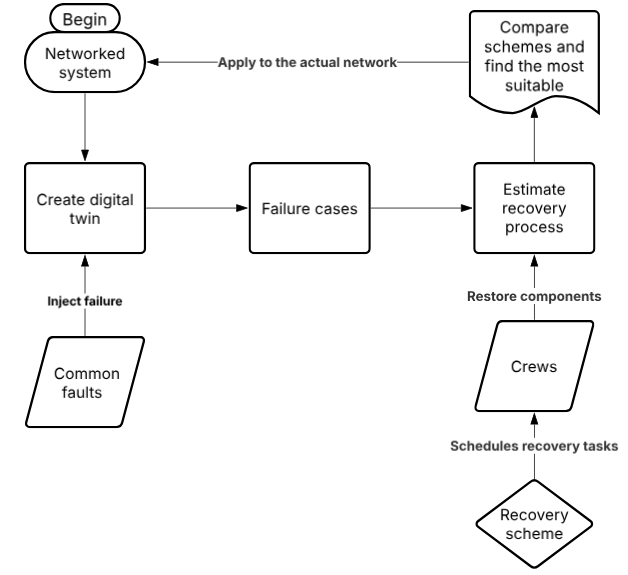
\includegraphics[width=0.7\linewidth]{images/methodology.png}
    \caption{Framework for comparing recovery schemes}
    \label{fig:methodology}
\end{figure}
\subsection{Recovery Schemes} 
We demonstrate the recovery model by applying it to the four recovery  schemes described below, which differ in how they prioritize components for recovery. 

\begin{enumerate}
\item The \emph{Randomized} scheme randomly selects a failed component at each decision epoch and assigns it to an available crew for recovery. 
\item The \emph{Precomputed} scheme uses (static) priority ordering that is computed beforehand. The priorities could be determined using component importance analysis \cite{alobaidi_survivability_2016}, expert opinion, or other methods. At each decision epoch, this scheme schedules recovery for the failed component that has the highest priority on the precomputed list. 
\item The \emph{Max-capacity} scheme is a dynamic prioritization scheme we adapted from the method proposed by Yan at el. \cite{yan_dynamic_2021}. Our scheme aims to increase service resilience by prioritizing the repair of components that achieve the greatest recovery rate for service capacity. 
Consider two system-level states, $\mathbf{x}_\tau$ and $\mathbf{x}_\gamma$, which reflect the same state for every component other than $i$. $\mathbf{x}_\tau$ reflects the failure of component $i$, i.e., $x_i = 1$. $\mathbf{x}_\gamma$ is identical to $\mathbf{x}_\tau$ in every other element, but $x_i = 0$. Let action $a$ represent the recovery of component $i$ in between these two states. The reward for this action represents the marginal effect of recovering component $i$ and is computed as the recovery rate of service capacity between these two states, as shown in Equation \ref{eq:Marginal-R}. In this equation, $E[T_{ri}]$ represents the expected repair time of component $i$, which is computed from historical data. 

\begin{equation}
    \text{Marginal effect of recovering }i = \frac{R_a(\mathbf{x}_\tau, \mathbf{x}\gamma)}{E[T_{ri}]}
    \label{eq:Marginal-R}
\end{equation}

\item The \emph{Min-cascade} scheme is a dynamic prioritization scheme we created for this research. This scheme aims to decrease the likelihood of failure propagation by prioritizing the repair of components most \emph{critical} to the system. In this context, a component's criticality is a measure of the number of other components it will bring down if it fails. This scheme considers two elements in calculating a \emph{cascading index} for each failed component, $i$. The first is the  expected number of currently operational components that will fail in the next time step as a result of $i$'s failure. This is the numerator of the fraction in Equation \ref{eq:min_cascade}. The second is $i$'s expected recovery time, $E[T_{ri}]$, which is the denominator of the fraction in Equation \ref{eq:min_cascade}. The component with the highest cascading index is selected for recovery. 
\begin{equation}
\label{eq:min_cascade}
\text{cascading index of } i 
= \frac{\sum_{j=1}^{N} d_{ij}*(1-x_j)}{E[T_{ri}]}
\end{equation}
\end{enumerate}

\begin{table}[!htbp]
  \centering
\caption{Summary of recovery schemes}
\label{table:recovery}
\begin{tabular}{|l|l|}
\hline
    \textbf{Schemes}                         & \textbf{Order of recovery tasks}    \\ \hline
    Randomized    & Random                               \\ \hline
    Precomputed                             & Computed beforehand                  \\ \hline
    Max-capacity \cite{yan_dynamic_2021}     & Aims to maximize recovered capacity   \\ \hline
    Min-cascade                              & Aims to minimize failure propagation  \\ \hline
\end{tabular}
\end{table}

Table \ref{table:recovery} provides a summary of the four recovery schemes. These schemes differ in computational complexity. The randomized scheme requires minimal computational resources compared to the others, as it randomly chooses a repair task for the next idle crew. In our experiments, the Pre-Computed scheme was on average 10\% slower than Randomized. This is not surprising, given that the former requires searching a list. The two dynamic schemes, Max-capacity and Min-cascade, are considerably more complex, as they look ahead in time and predict failure propagation. In our experiments (described in Section \ref{sec:case}, Min-Cascade was on average 20\% slower than the Randomized scheme. Max-Capacity requires performance evaluation of the network; its computational complexity can be reduced by using a precomputed lookup table to determine the service capacity for each system-level state. We found it to be on average 60\% slower than Randomized despite our use of the table. 

\section{Case Studies}
\label{sec:case}
To demonstrate that our recovery process model can correctly differentiate between the recovery rate of different schemes, we present the results of three case studies. In the interest of brevity and clarity, all three cases assume the same underlying cyber-physical system structure - a smart grid based on the commonly used IEEE 14-bus test system (IEEE-14), depicted in Figure \ref{fig:IEEE14BUS}. 

\begin{figure*}[!htbp]
    \centering
    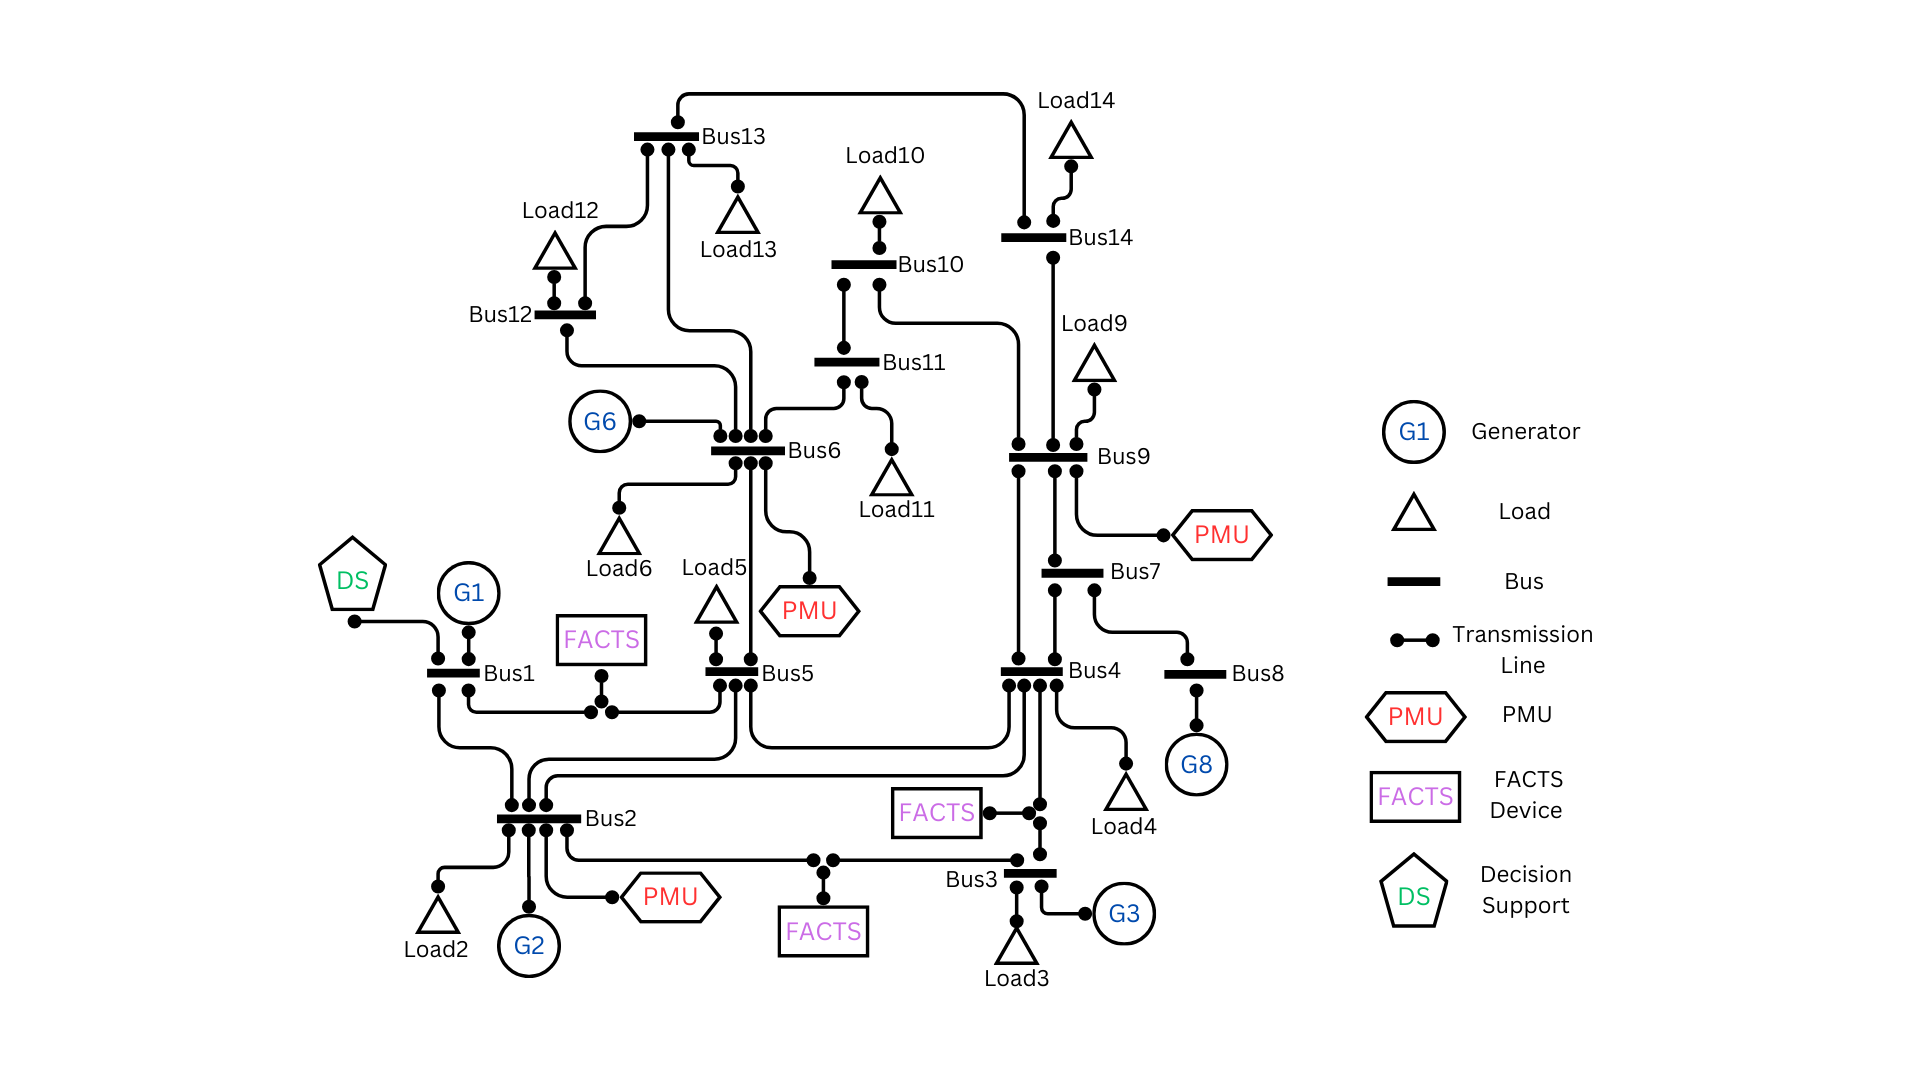
\includegraphics[width=1.2\linewidth]{images/IEEE-14 smart}
    \caption{IEEE-14 smart grid (adapted from \cite{marashi_identification_2021})}
    \label{fig:IEEE14BUS}
\end{figure*}

The original IEEE-14 includes five generators, twenty transmission lines, fourteen buses, and eleven loads. 
We have created an IEEE-14 smart grid from the original physical system by adding three phasor measurement units (PMUs),  three Flexible Alternating Current Transmission System (FACTS) devices, and a decision support system. The PMUs, which are high-speed sensors that carry out time-synchronized monitoring of voltages and currents on a power grid, were placed on buses 2, 6, and 9, respectively. These are the locations identified in a study by Asprou and Kyriakides ~\cite{asprou_optimal_2011} as leading to the most accurate estimates of the state of the grid. FACTS devices are used to control power flow and increase stability in power grids. They are widely used in the construction of smart grids \cite{sosnina_assessment_2022} and offer advantages over mechanical switching devices ~\cite{garrido_location_2019}. We added three FACTS devices to the IEEE-14 grid, on the lines between buses 1 and 5, 2 and 3, 3 and 4, respectively. The locations were recommended by Acharya and Mithulananthan  ~\cite{acharya_locating_2007} to achieve the highest stability in voltage and power factor. Finally, the decision support system was added to bus 1, which connects to the generator that typically provides the greatest fraction of the power. The role of the decision support system is to determine optimal settings for the FACTS device based on data from the PMUs. 
Among the physical components of the IEEE-14 smart grid, the focus of our analysis is on transmission lines, as they have higher failure rates as compared to other components and are often the cause of power outages \cite{song_survey_2013}. The failure of cyber components, i.e., PMUs, FACTS devices, and the decision support system, is also considered, as their malfunction can lead to cascading failure in an otherwise stable grid \cite{FaS10a}. 

A total of 27 components are considered for recovery, hence $N = 27$. 
The system-level state, $\mathbf{x}$, is represented as in Equation \ref{eq:X_cs}, where $\mathbf{x_i} = 1$ if component $i$ has failed.

\begin{equation}
    \mathbf{x} = \{x_1, x_2, \ldots , x_{27}\}
    \label{eq:X_cs}
\end{equation}

For the given IEEE-14 smart grid, the recovery time for each component is assumed to be uniformly distributed, ranging from 2 to 4 hours for a transmission line and 3 to 7 hours for the smart devices. These values have been assumed for illustrative purposes. Actual recovery times depend on the type of fault and can be inferred from historical data \cite{Vad17}. 


 %L- we can add this back if we have space
 %Then, the results are averaged to estimate the effectiveness of each recovery scheme against all cascading failures based on the likelihood of their occurrence. Each trial of simulation will be executed for 1,000 simulations, therefore each simulation representing 0.1\% of the possible outcome. The probability-based transitions (Equation \ref{eq:P}) will be determined by a random variate that is generated in the range of [0,1] uniformly.

\subsection{Simulation Environment}

The goal of the case studies is to show that the recovery scheme identified by the MDP can improve the delivered service capacity as compared to randomized assignment of recovery tasks, or prioritization that neglects the failure propagation that can be concurrent with recovery efforts. Our experiments were carried out using fault injection on PSAT ~\cite{psat_2005}, an open-source MATLAB-based toolbox for analysis of power systems, which we have modified to allow for simulation of interactions between components such as PMUs and the decision support algorithm that identifies settings for the FACTS devices. Our previous work \cite{MaS17c, marashi_identification_2021}  describes the simulation environment and explains how we ensured that cyber-physical interdependencies are accurately reflected in our experiments. 

%SSS - limitation of this work: all crews are considered equal. Let's make sure that we point this out. 
For each case study, our simulator requires three inputs: i) a description of the topology and specifications of the smart grid (including the recovery time distribution for each component) and 
ii) the number of crews available to restore the system. From this information, the simulator carries out power flow analysis to determine the active power flow on each line and the voltage at each bus. The phasor data is computed by the PMUs from this information and sent to the decision support system, which determines settings for the FACTS device, which in turn may regulate active and reactive power on the line where it is installed. A second round of power flow analysis by the simulator determines the result of this regulation and identifies overloaded lines and failed cyber components, reflecting failure propagation in the smart grid. A failed component remains failed until a repair crew completes its recovery. 

The MDP was formulated and solved in Python 3 on Google colab \cite{colab}, with three inputs: i) the dependency matrix (described in Section \ref{sec:mdp}) that governs transition probabilities and reflects cascading failure, ii) the recovery time distribution for each component, and iii) a look-up table that shows the service capacity, $SCI_\tau$ (defined in Equation \ref{eq:ServiceLoss}) for each system-level state, $\mathbf{x_\tau}$. In our case studies, the SCI is determined by the fraction of loads that are connected to buses operating within the expected voltage range. The expected range is 0.9 to 1.1 per-unit, where the per-unit representation denotes normalization by the base voltage of each bus. Pre-computing the SCI values increases the efficiency of the simulation. %The MDP was solved using the ``CPU'' option as the hardware accelerator with 12.7 GB RAM space.
%I removed the decision analysis section and replaced it with the following section
\subsection{IEEE-14 Failure Cases}
The assumptions underlying our model are described in Section \ref{sec:model}. One of them is that component states are observable, i.e., the failure of a component will be detected and repair efforts initiated quickly. Given that single-failure contingencies are the most probable, in a short-sighted approach, repair crews are likely to be dispatched to the first component whose failure is detected. However, given that an initial failure can propagate to other components, prediction of failure sequences could lead to more prudent dispatch of repair crews. 

Among the components in the smart grid, transmission lines, PMUs, FACTS devices, and the decision support system are the ones most likely to fail \cite{song_survey_2013}. The respective failure of each of these 27 components is the triggering event for one of the 27 failure cases analyzed in our case study. For each failure case, we ran 2,000 Monte Carlo simulation trials with a respective recovery time horizon of 100 hours and compared the number of cascading failures, time to first recovery, and service capacity achieved by each of the four recovery schemes summarized in Table \ref{table:recovery}. The \emph{time to first recovery} refers to the duration between injection of the failure and when all failed components have been repaired. The system may experience additional failures after this first recovery. Three separate experiments were conducted, with three, four, and five recovery crews, respectively.

\noindent\emph{Experiment 1: Three recovery crews available}\\
In the first experiment, we compared the four recovery schemes as respectively carried out by a total of three recovery crews. Failures can propagate as repair or replacement is being carried out, leading to cascading failures that could have been prevented by faster recovery efforts. In this experiment, as expected, the recovery scheme designed to reduce cascading failure outperforms the others. Table \ref{tab:3crews} summarizes the results of the experiment.
\begin{table}[!htbp]
\centering
\caption{Comparison of recovery schemes, three crews}
\label{tab:3crews}
\begin{tabular}{|c|c|c|}
\hline
\textbf{Scheme}       & Avg. time to first recovery (h) & Avg. number of cascading failures \\ \hline
\textbf{Randomized}   & 20.4         & 14.4            \\ \hline
\textbf{Precomputed} & 17.4         & 14.1            \\ \hline
\textbf{Max-capacity} & 19.6         & 14.7            \\ \hline
\textbf{Min-cascade}  & 17.7         & 12.7            \\ \hline
\end{tabular}
\end{table}

\begin{figure}
    \centering
    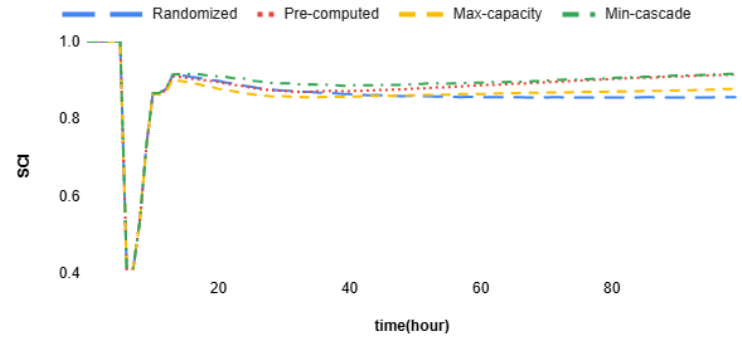
\includegraphics[width=0.7\linewidth]{images/compact_view.png}
    \caption{Comparison of service capacity, three crews}
    \label{fig:compact}
\end{figure}

Figures \ref{fig:compact} and \ref{fig:SCI-3} compare the service capacity achieved by the four recovery schemes. Min-cascade and  Precomputed were able to reduce the number of cascading failures and the average time it takes to restore the entire system. The Randomized scheme performs poorly by both metrics. The greedy approach taken by Max-capacity backfires, as recovery cannot keep up with failure propagation. The Min-cascade scheme maintained the highest service capacity for the largest fraction of the time horizon. Reducing the chance of cascading failure buys more time to request additional recovery resources. %SSS -see if we can improve wording of final sentence

\begin{figure*}[!htbp]
    \centering
    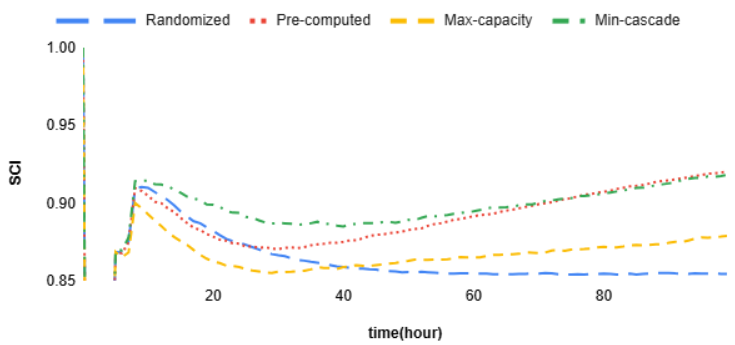
\includegraphics[width=.7\linewidth]{images/SCI-3crews.png}
    \caption{Focused view of service capacity during recovery, three crews}
    \label{fig:SCI-3}
\end{figure*}
\begin{comment}
For greater clarity, Figure \ref{fig:diff-3} illustrates the normalized performance ratio between each scheme and the randomized scheme, calculated as in Equation \ref{eq:ratio}. 

\begin{equation}
    \frac{\Delta}{\Delta_0}(\tau) = \frac{\text{SCI using recovery scheme at time}(\tau)}{\text{SCI using randomized scheme at time}(\tau)}
    \label{eq:ratio}
\end{equation}
\end{comment}
% \begin{figure*}[!htbp]
%     \centering
%     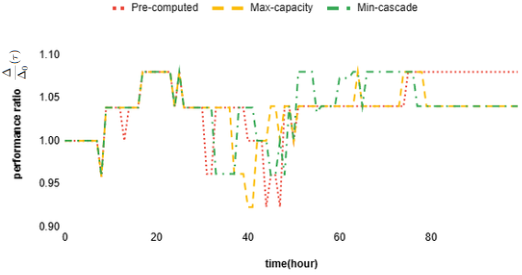
\includegraphics[width=.7\linewidth]{images/diff-3crews.png}
%     \caption{Normalized performance ratio vs. randomized recovery, three crews}
%     \label{fig:diff-3}
% \end{figure*}


\noindent\emph{Experiment 2: Four recovery crews available}\\
In the second experiment, four crews were assumed to be available. Table \ref{tab:4crews} summarizes the results of the experiment. As expected, both the time to first recovery and the number of cascading failures decrease when more hands are on deck. Figure \ref{fig:SCI-4} compares the service capacity achieved by each of the four schemes during the recovery process. Overall, the Min-cascade scheme shows the greatest efficacy. In comparison to experiment 1, the SCI is more stable and less degradation is experienced by users, especially in the Randomized and Max-capacity schemes, respectively. 
% The pre-computed and the Min-cascading schemes are able to keep the SCI almost the same as the previous case. %SSS - this is comparing to five crews
\begin{table}[!htbp]
\centering
\caption{Comparison of recovery schemes, four crews}
\label{tab:4crews}
\begin{tabular}{|c|c|c|}
\hline
\textbf{Scheme}       & Avg. time to first recovery (h) & Avg. number of cascading failures \\ \hline
\textbf{Randomized}   & 14.1  & 13.0      \\ \hline
\textbf{Precomputed} & 14.2  & 14.8      \\ \hline
\textbf{Max-capacity} & 14.5  & 12.3      \\ \hline
\textbf{Min-cascade}  & 13.3  & 11.0      \\ \hline
\end{tabular}
\end{table}

\begin{figure}[!htbp]
    \centering
    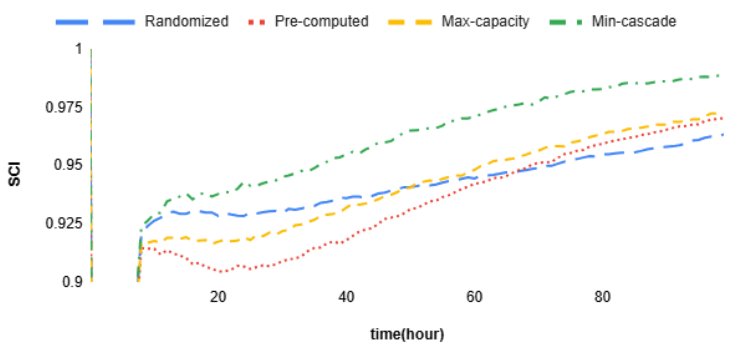
\includegraphics[width=.7\linewidth]{images/SCI-4crews.png}
    \caption{Comparison of service capacity, four crews}
    \label{fig:SCI-4}
\end{figure}

% \begin{comment}
% \begin{figure}[!htbp]
%     \centering
%     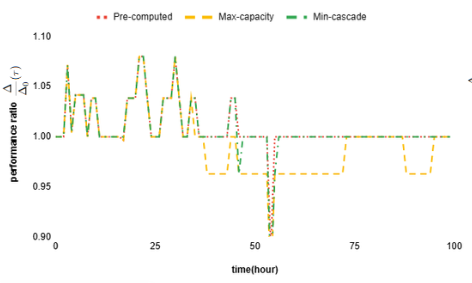
\includegraphics[width=.7\linewidth]{images/diff-4crews.png}
%     \caption{difference gap between each scheme vs. randomized}
%     \label{fig:diff-4}
% \end{figure}
% \end{comment}

\noindent\emph{Experiment 3: Five recovery crews available}\\
In the third experiment, we assume abundant recovery resources, i.e., the availability of five recovery crews. Given the size of the IEEE-14, having five crews available for recovery is admittedly unlikely to occur in reality, but useful in comparing how the number of crews affects  recovery. 
Table \ref{tab:5crew} summarizes the results of the experiment. The results indicate that the Max-capacity and Min-cascade schemes can achieve the quickest recovery time and the least cascading failures. Their time to first recovery is similar. This is not surprising, given that both of them dynamically adapt to the consequences of failure and recovery. 
\begin{table}[!htbp]
\centering
\caption{Comparison of recovery schemes, five crews available}
\label{tab:5crew}
\begin{tabular}{|c|c|c|}
\hline
\textbf{Scheme}       & Avg. time to first recovery (h) & Avg. number of cascading failures \\ \hline
\textbf{Randomized}   & 12.2 & 11.5    \\ \hline
\textbf{Precomputed} & 13.4 & 16.0    \\ \hline
\textbf{Max-capacity} & 11.9  & 11.0   \\ \hline
\textbf{Min-cascade}  & 11.8 & 11.0    \\ \hline
\end{tabular}
\end{table}
Figure \ref{fig:sci-5} compares the service capacity achieved by the four recovery schemes. We observe that the initial failure can quickly bring down more than three lines of the system, leaving it defunct for a very short time. The abundance of repair crews allows for rapid recovery. 

%of the  here, because they were both designed based on dependency index between the component, but the dynamic one was able to utilize the crews much better to achieve a better result. 
% Where the pre-computed was suffering from more cascading failure but still be able to maintain the system at nominal performance. The randomized scheme has the slowest recovery rate, it is the last one to bring the system back to nominal state, but it's very stable and did not suffer from cascading failures as much. Because in this scenario the system has 5 crews, much more than usual, the randomized scheme can assign them into random tasks, so fewer crews would be idle in comparison to the guided schemes. 
% For greater clarity, Figure \ref{fig:diff-5} illustrates the normalized performance ratio between each scheme and the randomized scheme, calculated as in Equation \ref{eq:ratio1} 

% \begin{equation}
%     \frac{\Delta}{\Delta_0}(\tau) = \frac{\text{SCI using recovery scheme at time}(\tau)}{\text{SCI using randomized scheme at time}(\tau)}
%     \label{eq:ratio1}
% \end{equation}. 
%Figures \ref{fig:avg-res-time} and \ref{fig:avg-cas-fai}, respectively, show to t 

%SSS - we need to sort out the results of the five-crew experiment. The text does not match the figure or table and the dynamic schemes seem to be underperforming. 


\begin{figure*}[!htbp]
    \centering
    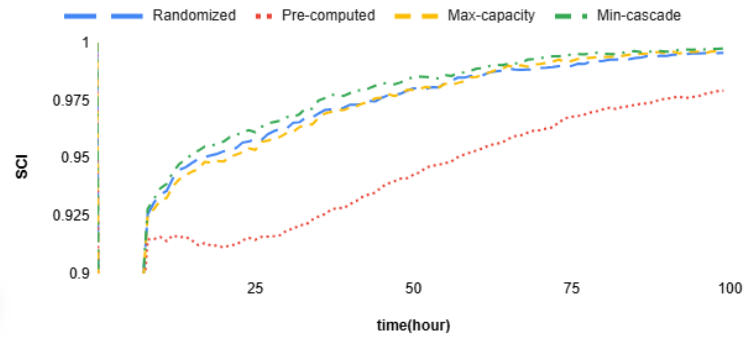
\includegraphics[width=.7\linewidth]{images/SCI-5crews.png}
    \caption{Comparison of service capacity, five crews}
    \label{fig:sci-5}
\end{figure*}

\begin{comment}
\begin{figure*}[!htbp]
    \centering
    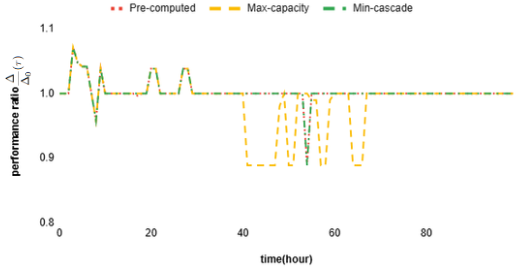
\includegraphics[width=.7\linewidth]{images/diff-5crews.png}
    \caption{Normalized performance ratio vs. randomized recovery}
    \label{fig:diff-5}
\end{figure*}

\end{comment}

Tables \ref{tab:recoverytime} and \ref{tab:failures} summarize the results of the 12 experiments, respectively comparing the average time to first recovery and average number of cascading failures for the four recovery schemes for different numbers of available crews. Overall, the Min-cascade scheme is found to be superior, achieving low time to first recovery and the lowest number of cascading failures. 

\begin{table}[!htbp]
\centering
\caption{Avg. time to first recovery for each scheme}
\label{tab:recoverytime}
\begin{tabular}{|c|c|c|c|c|}
\hline
\textbf{Crews} & \textbf{Randomized} & \textbf{\begin{tabular}[c]{@{}c@{}}Precomputed\end{tabular}} & \textbf{Max-capacity} & \textbf{\begin{tabular}[c]{@{}c@{}}Min-cascade\end{tabular}} \\ \hline
3    & 20.4       & 17.4       & 19.6       & 17.7   \\ \hline
4    & 14.1       & 14.2       & 14.5       & 13.3   \\ \hline
5    & 12.2       & 13.4       & 11.9       & 11.8   \\ \hline
\end{tabular}
\end{table}

\begin{table}[!htbp]
\centering
\caption{Avg. number of cascading failures for each scheme}
\label{tab:failures}
\begin{tabular}{|c|c|c|c|c|}
\hline
\textbf{crews} & \textbf{Randomized} & \textbf{\begin{tabular}[c]{@{}c@{}}Precomputed\end{tabular}} & \textbf{Max-capacity} & \textbf{\begin{tabular}[c]{@{}c@{}}Min-cascade\end{tabular}} \\ \hline
3    & 14.4       & 14.1        & 14.7      & 12.7   \\ \hline
4    & 13.0       & 14.8        & 12.3      & 11.0   \\ \hline
5    & 11.5       & 16.0        & 11.0      & 11.0   \\ \hline
\end{tabular}
\end{table}

\begin{comment}
\begin{table}[!htbp]
\centering
\caption{Recovery success rate before the end of time horizon (100 h)}
\label{tab:success rate}
\begin{tabular}{|c|c|c|c|c|}
\hline
\textbf{crews} & \textbf{Randomized} & \textbf{\begin{tabular}[c]{@{}c@{}}Precomputed\end{tabular}} & \textbf{Max-capacity} & \textbf{\begin{tabular}[c]{@{}c@{}}Min-cascade\end{tabular}} \\ \hline
3    & 85.0\%       & 91.9\%        & 91.8\%      & 91.3\%   \\ \hline
4    & 94.4\%       & 96.8\%        & 95.9\%      & 97.8\%   \\ \hline
5    & 98.7\%       & 97.6\%        & 99.0\%      & 99.0\%   \\ \hline
\end{tabular}
\end{table}
\end{comment}

\section{Conclusions}
This paper proposes a Markov decision process model for analysis and optimization of the recovery process of a complex networked system. We also propose two dynamic recovery schemes that predict and adapt recovery efforts to the consequences of failure propagation. The first scheme, adapted from \cite{yan_dynamic_2021}, aims to achieve the quickest possible recovery of service capacity. The second scheme aims to minimize cascading failure.  In a case study on the IEEE-14 smart grid, we compared the efficacy of the dynamic schemes to a randomized and a static scheme, respectively, for three scenarios that differ in the availability of repair resources (recovery crews). The results showed that each dynamic scheme achieved the objective for which it was designed. The Min-cascade scheme was the best overall, in terms of both time to first recovery and number of cascading failures. 

%In the case study, we found that when recovering a complex networked system from failures, cascading failure could bring down the system and even cause it to fall apart. Among the recovery process, the decisions to assign repair crews to work on each component of the system could be a difficult task, and it can affect the recovery process. We demonstrate the model by applying four different recovery schemes to 27 common failure cases. In each experiment, a different number of crews was assumed to be available throughout the entire recovery process for scenarios that has excessive recovery resource and the ones with a shortage. 

The immediate future work of this research is to validate scalability of the model by applying it to larger smart grids, e.g., IEEE-34 and 57, as well as complex networked systems from other application domains. Other future extensions include the following:
\begin{description}
    \item[Relaxing the assumption of observability of states]: Considering the effect of incomplete or uncertain information about the state of each component would be a closer representation of reality. 
    \item [Considering additional recovery schemes] We compared four schemes in this study. Several others have been demonstrated in respective case studies by Yan et al. \cite{yan_dynamic_2021} and Sarkale et al. \cite{sarkale_solving_2018}. Insights can be gained by comparing their efficacy.
    \item [Considering other performance metrics] Other than the loss in service capacity, there are many other ways to evaluate the performance of a complex networked system. Domain-specific examples include the stability of bus voltages and the cost of power production/distribution/storage. These metrics could be used as the basis for comparing the efficacy of recovery schemes. A multidimensional metric could yield insight about tradeoffs. 
    \item [Packaging and prototyping] A user-friendly interface to the model would make its real-time decision support accessible to system operators.

\end{description}


\section{Acknowledgements}
The authors gratefully acknowledge funding from NSF DUE-2221559 and DEd GAANN award  P200A210121. We extend our warmest thanks to Mr. John Czaicki, former Vice President of Quanta Utility Engineering Services, for sharing his professional insights.
\pagebreak

%\IEEEtriggeratref{6}

\bibliographystyle{IEEEtran}
\bibliography{export-data.bib}

\end{document}
